\section{Sensor NTC}

Nesta secção será descrito o funcionamento do sensor bem como a implementação do mesmo no circuito com o microcontrolador baseado na plataforma \textit{Arduino}.

O sensor NTC consiste num sensor térmico na qual a variação de temperatura traduz-se num valor de resistência que por sua vez é inversamente proporcional à variação da temperatura, daí ser denominada por \textit{Negative Temperature coefficient}. Este sensor é considerado um termístor.
\begin{figure}[!htb]
	\centering
	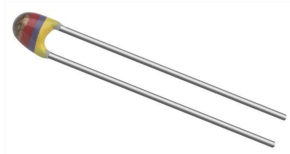
\includegraphics[width=0.3\textwidth]{img/NTC.PNG}
	\caption{Aspecto físico de um termístor NTC.}
	\label{fig:NTCsensor}
\end{figure}

Este sensor possui uma variação de resistência, como mencionado anteriormente. Para a escolha do sensor tem de se verificar na folha de especificações a gama de medições de temperatura que o sensor possibilita e a tolerância do sensor. Em seguida, escolhe-se o valor da resistência para o valor de referência para 25ºC consoante a tolerância do sensor.

Para a integração do sensor num circuito, elabora-se um circuito divisor resistivo com o sensor e a resistência que estabelece o valor de referência para 25ºC, como representa a Figura \ref{fig:NTCmontagem}
\begin{figure}[!htb]
	\centering
	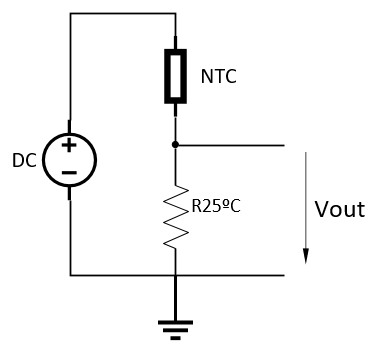
\includegraphics[width=0.3\textwidth]{img/NTCmontagem.PNG}
	\caption{Divisor resistivo com o sensor e a resistência que estabelece o valor de referência para 25ºC.}
	\label{fig:NTCmontagem}
\end{figure}

Para a obtenção de um valor de temperatura exato é necessário obedecer a alguns parâmetros impostos pelo sensor, sendo estes as constantes \(A_1\), \(B_1\) [\(k^{-1}\)], \(C_1\) [\(k^{-2}\)] e \(D_1\) [\(k^{-3}\)]. Após se ter obtido o valor dos parâmetros mencionados recorre-se á equação \ref{eq:Temperatura} na qual serão utilizados os valores dos parâmetros.
\begin{equation}
T [ºC] = \frac{1}{A_1 + B_1*\ln\frac{R}{R_{ref}} + C_1*\ln^2\frac{R}{R_{ref}} + D_1*\ln^3\frac{R}{R_{ref}}}- 273.15
\label{eq:Temperatura}
\end{equation}

É de notar que é subtraído à equação 273.15 para a conversão da temperatura de Kelvin para graus centígrados.

Uma das questões impostas no guião do trabalho de laboratório, é gama total de medição de temperatura que o sensor possibilita. A gama de medição é limitada pela tensão máxima que a entrada analógica da placa de desenvolvimento possibilita, sendo esta 5V DC. 

\newpage
